% !TeX root = ../main.tex

% \appendixtoc
% \appendix
% \ohead[]{\textsc{Appendix}}
\label{app:appendix}

% \renewcommand\thechapter{\roman{chapter}}
% \setcounter{chapter}{0}

% \pagebreak
% \includepdf[pages=-,scale=.9,pagecommand={}]{Aufgabenstellung.pdf} 
% PDF um 10% verkleinert einbinden --> Kopf- und Fußzeile  werden so korrekt dargestellt. Die Option `pages' ermöglicht es, eine bestimmte Sequenz von Seiten (z.B. 2-10 oder `-' für alle Seiten) auszuwählen.
% \pagebreak
%\includepdf[pages=-,scale=.8,pagecommand=\section*{A. eventGenerator.py}]{../appendix/eventGenerator.py.pdf}
%\includepdf[pages=-,scale=.8,pagecommand=\section*{B. sendEvents.py}]{../appendix/sendEvents.py.pdf}


% \RedeclareSectionCommand[beforeskip=\kapitelabstand         ]{chapter}


%%%%%%%%%%%%%%%%%%%%%%%%%%%%%%%%%%%%%%%%%%

%%%%%%%%%%%%%%%%%%%%%%%%%%%%%%%%%%%%%%%%%%
%%%%%%%%%%%%%%%%%%%%%%%%%%%%%%%%%%%%%%%%%%
\chapter{Fundamentals}

\section{Comparison of Trigonometric Functions}
\label{app:trogonometric-func-comp}

\begin{figure}[htbp!]
    \centering
    % \missingfigure{Comparison Tan, Cos, and Sin}
    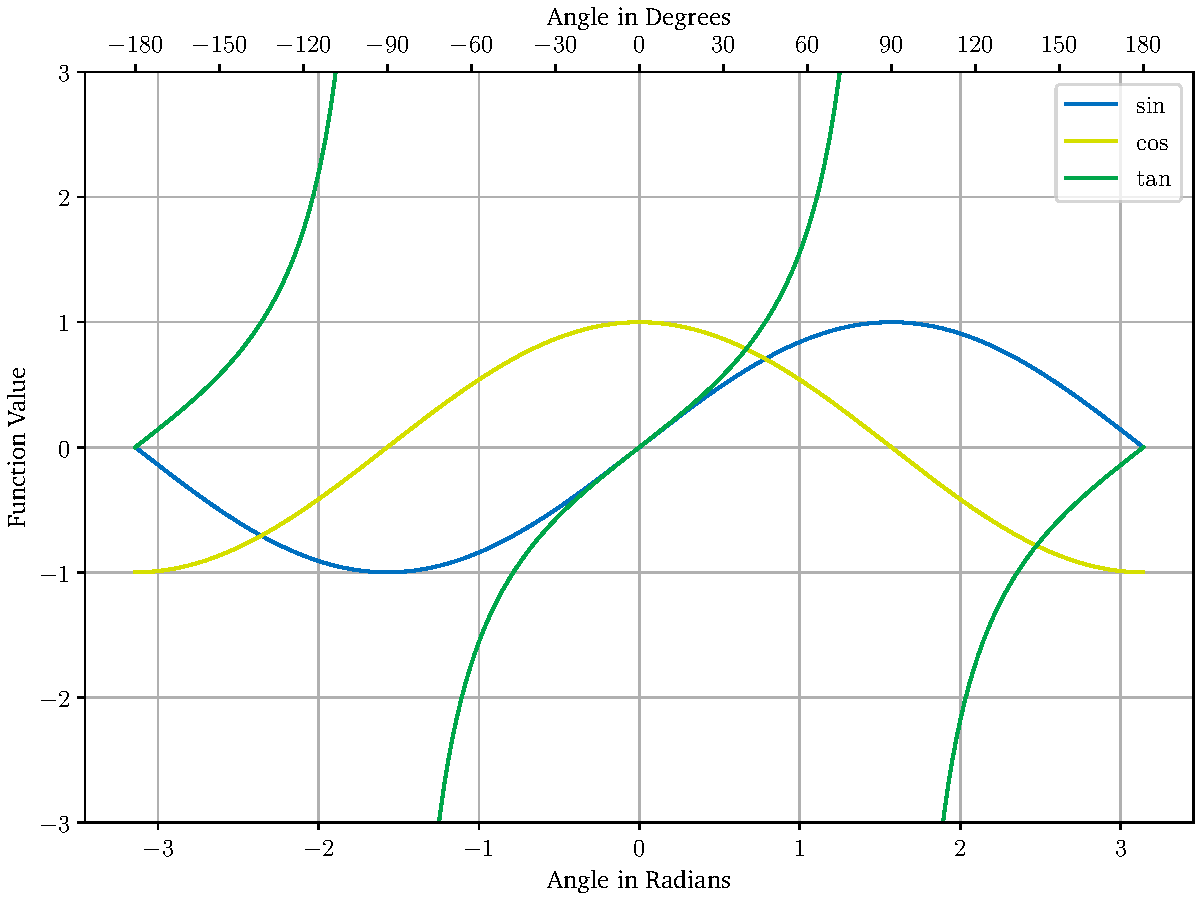
\includegraphics[width=\linewidth]{plots/trigonometric_functions.pdf}
    \caption[Plot comparison of trigonometric functions]{Plot comparison of trigonometric functions}
    \label{fig:trigonometric-func}
\end{figure}

\begin{table}[htbp!]
    \centering
    \small
    \caption{Comparison of trigonometric functions dependent on the angle $\phi$ in degree or radians}
    \vspace*{12pt}
    \begin{tabularx}{\linewidth}{XXXXX}
        \textbf{Angle in $^\circ$} & \textbf{Angle in rad} & \textbf{$\sin$} & \textbf{$\cos$} & \textbf{$\tan$} \\ \toprule
        0   & 0         & 0         & 1         & 0 \\
        10  & 0.1745    & 0.1736    & 0.9848    & 0.1763 \\
        20  & 0.3490    & 0.3420    & 0.9397    & 0.3640 \\
        30  & 0.5236    & 0.5       & 0.8660    & 0.5774 \\
        40  & 0.6981    & 0.6428    & 0.7660    & 0.8391 \\
        50  & 0.8727    & 0.7660    & 0.6428    & 1.1918 \\ 
        60  & 1.0472    & 0.8660    & 0.5       & 1.7321 \\
        70  & 1.2217    & 0.9397    & 0.3420    & 2.7475 \\
        80  & 1.3962    & 0.9848    & 0.1736    & 5.6713 \\
        90  & 1.5708    & 1         & 0         & $\nexists$ \\
        120 & 2.0944    & 0.8660    & -0.5      & -1.7321 \\
        150 & 2.6180    & 0.5       & -0.8660   & -0.5774 \\
        180 & 3.1416    & 0         & -1        & 0 \\
        \bottomrule
    \end{tabularx}
\end{table}

\section{Description of the Power System Simulation process}
\label{app:power-system-modeling}

In this appendix section, the general process of power system simulation is described. As this thesis is aiming to understand voltage stability and processes in longer periods of time, these explanations apply to pointer-based simulations, called RMS simulations. Meaning that the considered effects are slower electromechanical nature instead of faster electromagnetic ones. The in this thesis used Python framework \glqq \textit{diffpssi}\grqq~is based on this type of simulation, and due to its open-source based nature traceable.

\begin{figure}[htbp!]
    \centering
    % \includegraphics[width=\textwidth]{fundamentals/power-system-simulation-process.pdf}
    \missingfigure{Power system simulation process}
    \caption{Power system simulation process; own illustration}
    \label{fig:power-system-simulation-process}
\end{figure}

\commenting{
    Really basic: (?)
    \begin{itemize}
        \item RMS vs EMT simulation (-> meaning one cannot simulate other faults than 3ph w/o ground)
        \item Phasor description
        \item Basic formulation: Static (algebraic) and dynamic (differential) equations
        \item Using of solvers (Integrators) for time domain simulation
        \item Using of different optimizatinon algorithms for steady state (load flow) simulation -> initial values
    \end{itemize}
    Less basic and more advanced:
    \begin{itemize}
        \item rountines in the framework
        \item two types: Algebraic and Differential equations have to be solved at each time step -> What is which? Which operational equipment is typically described with which type of equation?
        \item per unit system applying for easier simulation (different voltage levels)
        \item ...
    \end{itemize}
}

%%%%%%%%%%%%%%%%%%%%%%%%%%%%%%%%%%%%%%%%%%
\section{Jacobian based voltage stability criterions}
\label{app:jacobian-voltage-indices}

\textcite{danish_2015} is showing, describing, and referencing some voltage stability indices based on the Jacobian matrix. The following table is a collection of these indices.

\begin{sidewaystable}[h]
    \centering
    \small
    \caption{Jacobian based voltage stability criterions; after \textcite{danish_2015}}
    \vspace*{12pt}
    \renewcommand{\arraystretch}{2}
    \begin{tabularx}{23cm}{llXXl}
        % \toprule
        \textbf{Index} & \textbf{Abbreviation} & \textbf{Calculation} & \textbf{Stability Threshold} & \textbf{Reference} \\
        \toprule
        Tangent Vector Index & \acs{TVI} & $\mathrm{TVI}_i=\left\lvert \frac{\dd{V_i}}{\dd{\lambda}}\right\rvert^{-1}$ & depending on load increase & \\ \midrule
        Test Function & & $t_{cc}=\left\lvert e^T_c \cdot \mab{J} \times \mab{J}_{cc}^{-1} \cdot e_c\right\rvert$ & details are given in reference & \\ \midrule
        Second Order Index & $i$ & $i=\frac{1}{i_0} \cdot \sigma_\mathrm{max} \cdot \big( \dv{\sigma_\mathrm{max}}{\lambda_\mathrm{total}} \big)^{-1}$ & $i > 0$ & \\ \midrule
        Minimum Eigenvalue & & $\Delta V=\sum_{i} \frac{\xi_i\eta_i}{\lambda_i} \Delta Q$ & all eigenvalues should be positive & \\ \midrule
        Minimum Singular Value & & $\begin{bmatrix} \Delta \vartheta \\ \Delta V \end{bmatrix}=\mab{V} \sum^-1 \mab{U}^T \begin{bmatrix} \Delta F \\ \Delta G \end{bmatrix}$ & details are given in reference & \\ \midrule
        Predicting Voltage Collapse & & $\frac{V}{V_0}$ & the smallest index value & \\ \midrule
        Impedance Ratio & & $\frac{Z_ii}{Z_i}$ & $\frac{Z_ii}{Z_i} \leq 1$ & \\
        \bottomrule
    \end{tabularx}
\end{sidewaystable}



%%%%%%%%%%%%%%%%%%%%%%%%%%%%%%%%%%%%%%%%%%
\section{Comparison of System based and Jacobian based indices}
\label{app:jacobian-vs-system-indices}

% %%%%%%%%%%%%%%%%%%%%%%%%%%%%%%%%%%%%%%%%%%
% %%%%%%%%%%%%%%%%%%%%%%%%%%%%%%%%%%%%%%%%%%
\chapter{Modeling}

%%%%%%%%%%%%%%%%%%%%%%%%%%%%%%%%%%%%%%%%%%
\section{Admittance Calculation of a Two-Port}
\label{app:admittance-deduction}

Follwing part shall just give a short, but complete and clear overview, how the admittance matrix of a two-port system is calculated.
Therefore the main focus of this thesis, a two-port with variable translation ratio, is kept.

%%%%%%%%%%%%%%%%%%%%%%%%%%%%%%%%%%%%%%%%%%
\section{Class Diagram of the Class Nose Curves}
\label{app:nose-curve}

\begin{figure}[htbp!]
    \centering
    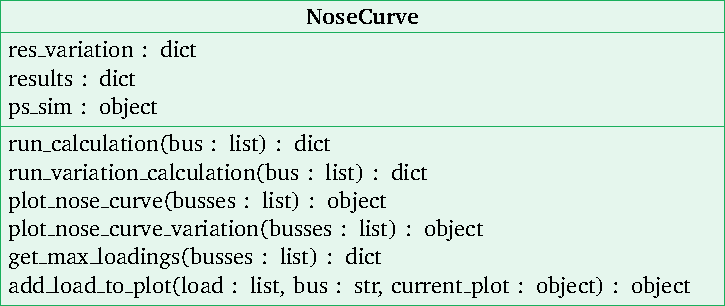
\includegraphics[width=12cm]{tikz_graphics/images/class_diagram_nosecurve_complete.pdf}
    \caption{Complete class diagram of the class Nose Curves; including all attributes and methods with data types, returns, and inputs}
    \label{fig:class-diagram-nose-curves}
\end{figure}

%%%%%%%%%%%%%%%%%%%%%%%%%%%%%%%%%%%%%%%%%%
\section{Analytical Calculation of Simple Nose Curves}
\label{app:analytical-nose-curve}

Some blibla and equations about the analytical calculation of simple nose curves.


%%%%%%%%%%%%%%%%%%%%%%%%%%%%%%%%%%%%%%%%%%
\section{Alternative Current Injection Model}
\label{app:current-injection-model}

\textcite{machowski_2020} describes another way of modeling a \acs{OLTC} transformer with variable ratio.
This model is looking at the shunt brnaches as current injections, which are added to the individual busses.
Beneficial, the system admittance matrix is staying symmetrical, while the different transformer state(s) are represented by the different current injections.
This can be mathematically expressed by following set of equations:
\begin{align}
    \begin{bmatrix}
        \underline{I}_1 \\
        -\underline{I}_2
    \end{bmatrix} &=
    \begin{bmatrix}
        \underline{Y}_\mathrm{T} & -\underline{Y}_\mathrm{T} \\
        -\underline{Y}_\mathrm{T} & \underline{Y}_\mathrm{T}
    \end{bmatrix}
    \begin{bmatrix}
        \underline{U}_1 \\
        \underline{U}_2
    \end{bmatrix} -
    \begin{bmatrix}
        \Delta \underline{I}_1 \\
        \Delta \underline{I}_2
    \end{bmatrix}\text{, where } \notag \\[12pt]
    \begin{bmatrix}
        \Delta \underline{I}_1 \\
        \Delta \underline{I}_2
    \end{bmatrix} &=
    \begin{bmatrix}
        \underline{0} & (\underline{\vartheta}-1)\underline{Y}_\mathrm{T} \\
        -(\underline{\vartheta}^*+1)\underline{Y}_\mathrm{T} & (\underline{\vartheta}^*\underline{\vartheta}+1)\underline{Y}_\mathrm{T}
    \end{bmatrix}
    \begin{bmatrix}
        \underline{U}_1 \\
        \underline{U}_2
    \end{bmatrix} \text{ leading to } \notag \\[12pt]
    \underline{\mab{Y}}_\mathrm{\Pi,T,Current~Injection}&= 
    \begin{bmatrix}
        \underline{Y}_\mathrm{T} & -\underline{Y}_\mathrm{T} \\
        -\underline{Y}_\mathrm{T} & \underline{Y}_\mathrm{T}
    \end{bmatrix} -
    \begin{bmatrix}
        \underline{0} & (\underline{\vartheta}-1)\underline{Y}_\mathrm{T} \\
        -(\underline{\vartheta}^*+1)\underline{Y}_\mathrm{T} & (\underline{\vartheta}^*\underline{\vartheta}+1)\underline{Y}_\mathrm{T}
    \end{bmatrix} \notag % \label{eq:admittance-oltc-2}
\end{align}

% %%%%%%%%%%%%%%%%%%%%%%%%%%%%%%%%%%%%%%%%%%
% \section{OLTC control}


% %%%%%%%%%%%%%%%%%%%%%%%%%%%%%%%%%%%%%%%%%%
% %%%%%%%%%%%%%%%%%%%%%%%%%%%%%%%%%%%%%%%%%%
% \chapter{Verification}

% %%%%%%%%%%%%%%%%%%%%%%%%%%%%%%%%%%%%%%%%%%
% \section{Single-machine infinite bus-bar model}
% \label{app:smib-model}


% %%%%%%%%%%%%%%%%%%%%%%%%%%%%%%%%%%%%%%%%%%
% %%%%%%%%%%%%%%%%%%%%%%%%%%%%%%%%%%%%%%%%%%
% \chapter{Case study}